\documentclass[12pt]{article}
\usepackage[utf8]{inputenc}
\usepackage{graphicx}
\usepackage{float}
\usepackage{amsmath}
\usepackage{amssymb}
\usepackage{tikz}
\usepackage{listings}
\usepackage{xcolor}
\usepackage{hyperref}
\usepackage{enumitem}
\usepackage{algorithm}
\usepackage{algpseudocode}

% Page layout
\usepackage[a4paper, margin=1in]{geometry}

% Colors
\definecolor{codegreen}{rgb}{0,0.6,0}
\definecolor{codegray}{rgb}{0.5,0.5,0.5}
\definecolor{codepurple}{rgb}{0.58,0,0.82}
\definecolor{backcolour}{rgb}{0.95,0.95,0.92}

% Code listing style
\lstdefinestyle{mystyle}{
    backgroundcolor=\color{backcolour},   
    commentstyle=\color{codegreen},
    keywordstyle=\color{blue},
    numberstyle=\tiny\color{codegray},
    stringstyle=\color{codepurple},
    basicstyle=\ttfamily\footnotesize,
    breakatwhitespace=false,         
    breaklines=true,                 
    captionpos=b,                    
    keepspaces=true,                 
    numbers=left,                    
    numbersep=5pt,                  
    showspaces=false,                
    showstringspaces=false,
    showtabs=false,                  
    tabsize=2
}
\lstset{style=mystyle}

% Title page variables
\title{EHB354E OBJECT ORIENTED PROGRAMMING PROJECT REPORT\\
SPRING 2025\\[2cm]
{\Large NEURAL NETWORK MNIST CLASSIFIER}\\[7cm]}

\author{Student Name: Kadir Yavuz Kurt \\
Student Number: 040240726}
\date{Date: \today}

\begin{document}

\maketitle
\newpage

\tableofcontents
\newpage

\section{Introduction}

This project implements a neural network-based classifier for the MNIST handwritten digit dataset. The MNIST (Modified National Institute of Standards and Technology) dataset is a large database of handwritten digits commonly used for training various image processing systems. The primary goals of the project include:

\begin{itemize}
    \item Developing a fully-functional neural network from scratch in C++
    \item Creating an interactive visual interface using SFML (Simple and Fast Multimedia Library)
    \item Implementing a system that allows users to build, train, and test neural networks on the MNIST dataset
    \item Demonstrating object-oriented design principles in a complex application
\end{itemize}

The application allows users to create custom neural network architectures by adding hidden layers, train the network on MNIST data, and test the network's performance. The visual interface provides real-time feedback on the network's structure and predictions, making it an educational tool for understanding neural network operations.

\section{Implementation}

\subsection{Class Structure}

The project implements a comprehensive object-oriented design with several key classes that interact to provide the full functionality of the neural network classifier. Each class has a specific responsibility, following the single responsibility principle.

\begin{figure}[H]
\centering
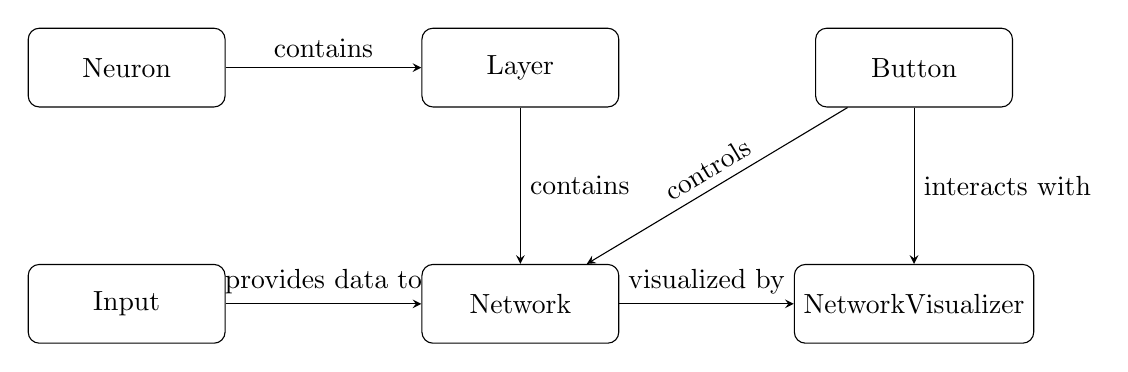
\begin{tikzpicture}[
    node distance=2cm,
    class/.style={draw, rectangle, rounded corners, minimum width=2.5cm, minimum height=1cm},
    arrow/.style={->, >=stealth}
]
    % Place nodes
    \node[class] (neuron) {Neuron};
    \node[class, right of=neuron, xshift=3cm] (layer) {Layer};
    \node[class, below of=layer, yshift=-1cm] (network) {Network};
    \node[class, left of=network, xshift=-3cm] (input) {Input};
    \node[class, right of=network, xshift=3cm] (visualizer) {NetworkVisualizer};
    \node[class, above of=visualizer, yshift=1cm] (button) {Button};
    
    % Add connections
    \draw[arrow] (neuron) -- (layer) node[midway, above] {contains};
    \draw[arrow] (layer) -- (network) node[midway, right] {contains};
    \draw[arrow] (network) -- (visualizer) node[midway, above] {visualized by};
    \draw[arrow] (input) -- (network) node[midway, above] {provides data to};
    \draw[arrow] (button) -- (visualizer) node[midway, right] {interacts with};
    \draw[arrow] (button) -- (network) node[midway, above, sloped] {controls};
\end{tikzpicture}
\caption{Class relationship diagram showing the main components of the application}
\label{fig:class_diagram}
\end{figure}

\subsubsection{Neuron Class}

The Neuron class represents an individual processing unit in the neural network. Each neuron:

\begin{itemize}
    \item Maintains weights for connections to the previous layer
    \item Has a bias term
    \item Computes its activation based on inputs
    \item Updates its weights during training
\end{itemize}

Key methods include:
\begin{lstlisting}[language=C++]
void computeOutput(const std::vector<double>& inputs);
double activate(double x) const;
void updateWeights(const std::vector<double>& inputs, double learningRate);
void calculateOutputDelta(double target);
void calculateHiddenDelta(const std::vector<Neuron>& nextLayer, size_t myIndex);
\end{lstlisting}

The class implements different activation functions, including ReLU and support for Softmax (implemented at the layer level).

\subsubsection{Layer Class}

The Layer class represents a collection of neurons that form a single layer in the neural network. It:

\begin{itemize}
    \item Manages a collection of Neuron objects
    \item Handles forward propagation through all neurons in the layer
    \item Implements special activations like Softmax for output layers
    \item Manages the backpropagation process for the layer
\end{itemize}

Key methods include:
\begin{lstlisting}[language=C++]
void forwardPropagate(const std::vector<double>& inputs);
void applySoftmax();
void calculateOutputLayerDeltas(const std::vector<double>& targets);
void calculateHiddenLayerDeltas(const Layer& nextLayer);
void updateWeights(double learningRate);
\end{lstlisting}

\subsubsection{Network Class}

The Network class is the central component that manages the entire neural network. It:

\begin{itemize}
    \item Maintains a collection of Layer objects
    \item Handles the addition of new layers to the network
    \item Manages forward propagation through the entire network
    \item Implements the complete training and testing processes
    \item Provides methods for data loading and preprocessing
\end{itemize}

Key methods include:
\begin{lstlisting}[language=C++]
void addLayer(size_t neuronCount, ActivationType type);
std::vector<double> forwardPropagate(const std::vector<double>& inputs);
double trainSingle(const std::vector<double>& inputs, const std::vector<double>& targets);
void train(const std::string& trainFile, int epochs, int batchSize);
double test(const std::string& testFile, int numSamples = -1);
int predict(const std::vector<double>& input);
\end{lstlisting}

\subsubsection{Input Class}

The Input class handles loading and preprocessing the MNIST data, as well as visualizing individual examples. It:

\begin{itemize}
    \item Loads MNIST data from CSV files
    \item Normalizes pixel values for neural network input
    \item Manages the current example being displayed
    \item Visualizes the handwritten digits using SFML
\end{itemize}

Key methods include:
\begin{lstlisting}[language=C++]
bool loadData(const std::string& filename, int maxSamples = -1);
std::vector<double> getCurrentImageVector() const;
int getCurrentLabel() const;
void updateImageDisplay();
void nextImage();
void prevImage();
void randomImage();
\end{lstlisting}

\subsubsection{Button Class}

The Button class implements an interactive UI element using SFML. It:

\begin{itemize}
    \item Creates clickable buttons with text
    \item Handles mouse events and state changes
    \item Executes callback functions when clicked
    \item Provides visual feedback for hover and press states
\end{itemize}

Key methods include:
\begin{lstlisting}[language=C++]
void update(const sf::Vector2i& mousePosition);
bool isMouseOver(const sf::Vector2i& mousePosition) const;
void handleMousePress();
void handleMouseRelease(const sf::Vector2i& mousePosition);
void setCallback(std::function<void()> func);
\end{lstlisting}

\subsubsection{NetworkVisualizer Class}

The NetworkVisualizer class creates a graphical representation of the neural network. It:

\begin{itemize}
    \item Visualizes the network structure with layers and neurons
    \item Shows connections between neurons
    \item Displays activation levels using color intensity
    \item Highlights the winning output neuron for classification tasks
\end{itemize}

Key methods include:
\begin{lstlisting}[language=C++]
void update(const std::vector<double>& input);
void draw(sf::RenderWindow& window) const;
void calculateNeuronPositions();
void updateNetworkStructure();
void setConnectionsVisible(bool visible);
\end{lstlisting}

\subsection{Neural Network Algorithm}

The implementation follows the standard neural network algorithm with a focus on feedforward neural networks. The main components of the algorithm are:

\begin{figure}[H]
\centering
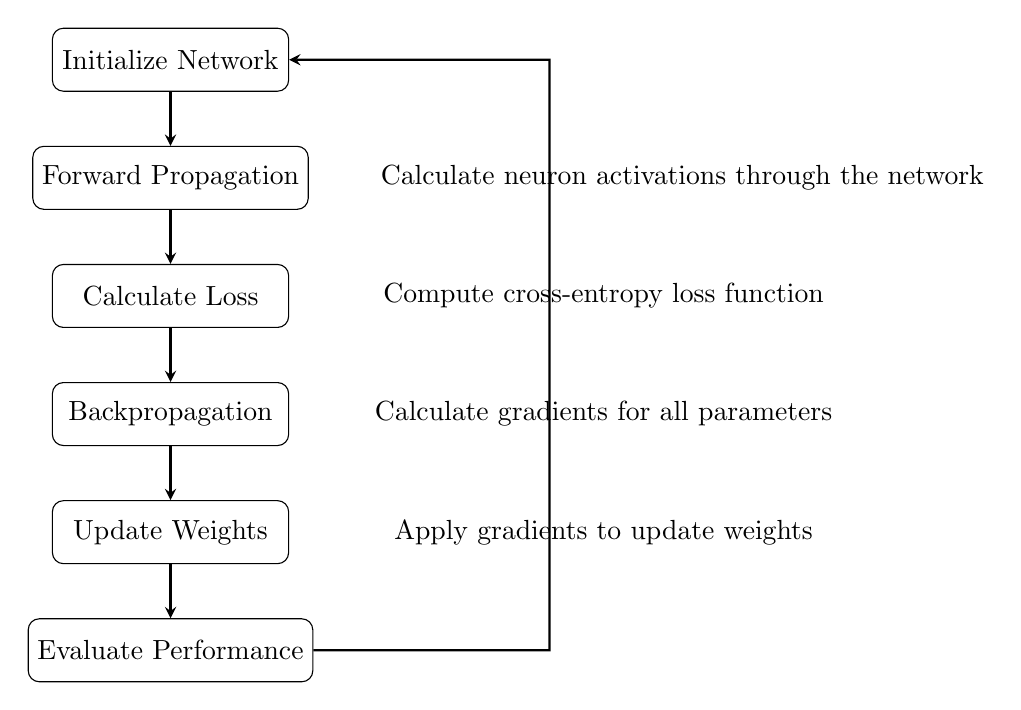
\begin{tikzpicture}[
    node distance=1.5cm,
    process/.style={draw, rectangle, rounded corners, minimum width=3cm, minimum height=0.8cm},
    arrow/.style={->, >=stealth, thick}
]
    % Nodes
    \node[process] (init) {Initialize Network};
    \node[process, below of=init] (forward) {Forward Propagation};
    \node[process, below of=forward] (loss) {Calculate Loss};
    \node[process, below of=loss] (backward) {Backpropagation};
    \node[process, below of=backward] (update) {Update Weights};
    \node[process, below of=update] (evaluate) {Evaluate Performance};
    
    % Connections
    \draw[arrow] (init) -- (forward);
    \draw[arrow] (forward) -- (loss);
    \draw[arrow] (loss) -- (backward);
    \draw[arrow] (backward) -- (update);
    \draw[arrow] (update) -- (evaluate);
    \draw[arrow] (evaluate.east) -- ++(3,0) -- ++(0,7.5) -- (init.east);

    % Labels
    \node[right of=forward, xshift=5cm] {Calculate neuron activations through the network};
    \node[right of=loss, xshift=4cm] {Compute cross-entropy loss function};
    \node[right of=backward, xshift=4cm] {Calculate gradients for all parameters};
    \node[right of=update, xshift=4cm] {Apply gradients to update weights};
\end{tikzpicture}

\caption{Neural Network Training Flow}
\label{fig:nn_flow}
\end{figure}

\subsubsection{Forward Propagation}

Forward propagation calculates the output of the network given an input. For each layer:

\begin{algorithm}
\caption{Forward Propagation}
\begin{algorithmic}[1]
\Procedure{ForwardPropagate}{$inputs$}
    \State $currentInputs \gets inputs$
    \For{each $layer$ in $network$}
        \For{each $neuron$ in $layer$}
            \State $sum \gets bias$
            \For{$i \gets 0$ to $inputs.size() - 1$}
                \State $sum \gets sum + inputs[i] \times weights[i]$
            \EndFor
            \State $output \gets activation(sum)$
        \EndFor
        \If{$layer$ is output layer}
            \State Apply Softmax activation
        \EndIf
        \State $currentInputs \gets layer.outputs$
    \EndFor
    \State \Return $currentInputs$
\EndProcedure
\end{algorithmic}
\end{algorithm}

\subsubsection{Backpropagation}

Backpropagation calculates the gradients of the loss function with respect to the network weights:

\begin{algorithm}
\caption{Backpropagation}
\begin{algorithmic}[1]
\Procedure{Backpropagate}{$inputs, targets$}
    \State $outputs \gets$ ForwardPropagate($inputs$)
    \State Calculate output layer deltas: $\delta_j = (target_j - output_j)$
    \For{$layer \gets network.size() - 2$ down to $0$}
        \For{each $neuron_i$ in $layer$}
            \State $\delta_i \gets 0$
            \For{each $neuron_j$ in $nextLayer$}
                \State $\delta_i \gets \delta_i + \delta_j \times weight_{ji}$
            \EndFor
            \State $\delta_i \gets \delta_i \times derivative(activation_i)$
        \EndFor
    \EndFor
    \For{each $layer$ in $network$}
        \For{each $neuron$ in $layer$}
            \For{each $weight$ of $neuron$}
                \State $weight \gets weight + learningRate \times \delta \times input$
            \EndFor
            \State $bias \gets bias + learningRate \times \delta$
        \EndFor
    \EndFor
\EndProcedure
\end{algorithmic}
\end{algorithm}

\subsubsection{Softmax Activation}

For the output layer, a softmax activation function is used to convert the raw outputs into a probability distribution:

\begin{equation}
\text{softmax}(x_i) = \frac{e^{x_i}}{\sum_{j} e^{x_j}}
\end{equation}

This implementation includes a numerical stability enhancement by subtracting the maximum value before applying the exponentiation:

\begin{lstlisting}[language=C++]
// Find max value for numerical stability
double maxOutput = -std::numeric_limits<double>::max();
for (const auto& neuron : neurons) {
    double output = neuron.getOutput();
    if (output > maxOutput) {
        maxOutput = output;
    }
}

// Calculate softmax with stability enhancement
double sumExp = 0.0;
for (double output : rawOutputs) {
    double expOutput = std::exp(output - maxOutput);
    expOutputs.push_back(expOutput);
    sumExp += expOutput;
}

// Apply softmax to each neuron
for (size_t i = 0; i < neurons.size(); i++) {
    double softmaxOutput = expOutputs[i] / sumExp;
    neurons[i].setOutput(softmaxOutput);
}
\end{lstlisting}

\subsection{Object-Oriented Programming Features}

The implementation showcases several key object-oriented programming features:

\subsubsection{Encapsulation}

The project extensively uses encapsulation to hide implementation details and provide controlled access to internal data:

\begin{itemize}
    \item Private member variables with public accessor methods
    \item Clear separation between interface and implementation
    \item Implementation details hidden within classes
\end{itemize}

Example from the Neuron class:
\begin{lstlisting}[language=C++]
private:
    std::vector<double> weights;  // Weights for connections to the previous layer
    double bias;                  // Bias term
    double output;                // Output value after activation
    double delta;                 // Error delta for backpropagation
    ActivationType activationType; // Type of activation function used
    
public:
    double getOutput() const;
    void setOutput(double val);
    double getDelta() const;
    void setDelta(double val);
    ActivationType getActivationType() const;
\end{lstlisting}

\subsubsection{Abstraction}

The implementation abstracts complex processes into simpler interfaces:

\begin{itemize}
    \item The Network class abstracts the entire neural network operation behind a simple interface
    \item The Layer class hides the details of managing multiple neurons
    \item The NetworkVisualizer class abstracts the complex visualization logic
\end{itemize}

For example, training the network is abstracted to a simple method call:
\begin{lstlisting}[language=C++]
network.train("data/mnist_data_train.csv", 1, 32);
\end{lstlisting}

\subsubsection{Composition}

The project uses composition to build complex objects from simpler ones:

\begin{itemize}
    \item Network is composed of Layers
    \item Layer is composed of Neurons
    \item NetworkVisualizer uses the Network's structure but doesn't inherit from it
\end{itemize}

This composition approach allows for more flexible and modular design.

\subsubsection{Polymorphism}

While not using inheritance hierarchies extensively, the project does use polymorphic behavior through function parameters and activation types:

\begin{itemize}
    \item The ActivationType enum class provides different activation behaviors
    \item The Button class uses std::function for callback functionality, allowing different behaviors for each button
\end{itemize}

Example from the Neuron class:
\begin{lstlisting}[language=C++]
double Neuron::activate(double x) const {
    switch (activationType) {
        case ActivationType::RELU:
            return std::max(0.0, x);
        case ActivationType::SOFTMAX:
            return x;
        default:
            throw std::runtime_error("Unknown activation type");
    }
}
\end{lstlisting}

\section{Challenges and Solutions}

\subsection{Numerical Stability in Neural Network Calculations}

\textbf{Challenge:} Neural networks are prone to numerical instability issues, particularly when dealing with activation functions like softmax that involve exponentiation.

\textbf{Solution:} Implemented a numerically stable version of the softmax function by subtracting the maximum value from all inputs before exponentiation:

\begin{lstlisting}[language=C++]
// Find max value for numerical stability
double maxOutput = -std::numeric_limits<double>::max();
for (const auto& neuron : neurons) {
    maxOutput = std::max(maxOutput, neuron.getOutput());
}

// Calculate softmax with stability enhancement
double sumExp = 0.0;
for (double output : rawOutputs) {
    double expOutput = std::exp(output - maxOutput);
    expOutputs.push_back(expOutput);
    sumExp += expOutput;
}
\end{lstlisting}

This prevents overflow when calculating exponentials while maintaining the same mathematical result.

\subsection{Visualization of Network Structure}

\textbf{Challenge:} Creating an intuitive visualization of a neural network with varying numbers of layers and neurons.

\textbf{Solution:} Developed an adaptive layout algorithm in the NetworkVisualizer class that calculates appropriate spacing and positions for neurons based on the network structure:

\begin{lstlisting}[language=C++]
void NetworkVisualizer::calculateNeuronPositions() {
    // Calculate appropriate spacing based on network structure
    const std::vector<Layer>& layers = network->getLayers();
    
    // Calculate layer spacing
    layerSpacing = size.x / (layers.size() + 1);
    
    // Update neuron positions for each layer
    neuronPositions.clear();
    for (size_t i = 0; i < layers.size(); ++i) {
        // Calculate appropriate spacing for neurons in this layer
        size_t neuronCount = layers[i].getNeuronCount();
        neuronSpacing = size.y / (neuronCount + 1);
        
        // Calculate positions for each neuron
        std::vector<sf::Vector2f> layerPositions;
        for (size_t j = 0; j < neuronCount; ++j) {
            float x = position.x + (i + 1) * layerSpacing;
            float y = position.y + (j + 1) * neuronSpacing;
            layerPositions.push_back(sf::Vector2f(x, y));
        }
        neuronPositions.push_back(layerPositions);
    }
}
\end{lstlisting}

This approach ensures that the visualization remains clear and informative regardless of the network's complexity.

\subsection{Data Handling and Preprocessing}

\textbf{Challenge:} Efficiently loading and preprocessing the MNIST dataset, which contains thousands of examples.

\textbf{Solution:} Implemented a streaming approach to data loading that processes the CSV files line by line, normalizing values and converting labels to one-hot encoded vectors:

\begin{lstlisting}[language=C++]
std::pair<std::vector<std::vector<double>>, std::vector<std::vector<double>>> 
Network::loadMNISTData(const std::string& filename, int numSamples) {
    std::ifstream file(filename);
    std::vector<std::vector<double>> inputs;
    std::vector<std::vector<double>> targets;
    
    std::string line;
    int count = 0;
    
    while (std::getline(file, line) && (numSamples == -1 || count < numSamples)) {
        std::stringstream ss(line);
        std::string value;
        
        // Read the label (first value in the row)
        std::getline(ss, value, ',');
        int label = std::stoi(value);
        
        // Convert label to target vector
        std::vector<double> target = labelToTarget(label);
        
        // Read pixel values (remaining values in the row)
        std::vector<double> input;
        while (std::getline(ss, value, ',')) {
            // Normalize pixel values to [0,1]
            double pixelValue = std::stod(value) / 255.0;
            input.push_back(pixelValue);
        }
        
        inputs.push_back(input);
        targets.push_back(target);
        count++;
    }
    
    return {inputs, targets};
}
\end{lstlisting}

This approach allows for efficient memory usage and supports loading subsets of the data for quick testing.

\subsection{Interactive User Interface Design}

\textbf{Challenge:} Creating an intuitive, responsive user interface that allows users to interact with the neural network.

\textbf{Solution:} Implemented a component-based UI system using SFML, with the Button class acting as the primary interactive element. Each button has a callback function that performs specific actions when clicked:

\begin{lstlisting}[language=C++]
buttons.emplace_back(
    sf::Vector2f(50, 400), sf::Vector2f(200, 40), 
    "Add Hidden Layer", &font, 
    [&]() {
        network.addLayer(16, ActivationType::RELU);
        statusText.setString("Status: Added hidden layer with 16 neurons");
        visualizer.updateNetworkStructure();
    }
);
\end{lstlisting}

The use of lambda functions allows for concise, context-specific button behaviors while maintaining a clean separation of concerns.

\section{Conclusion and Future Enhancements}

\subsection{Conclusion}

\begin{figure}[H]
    \centering
    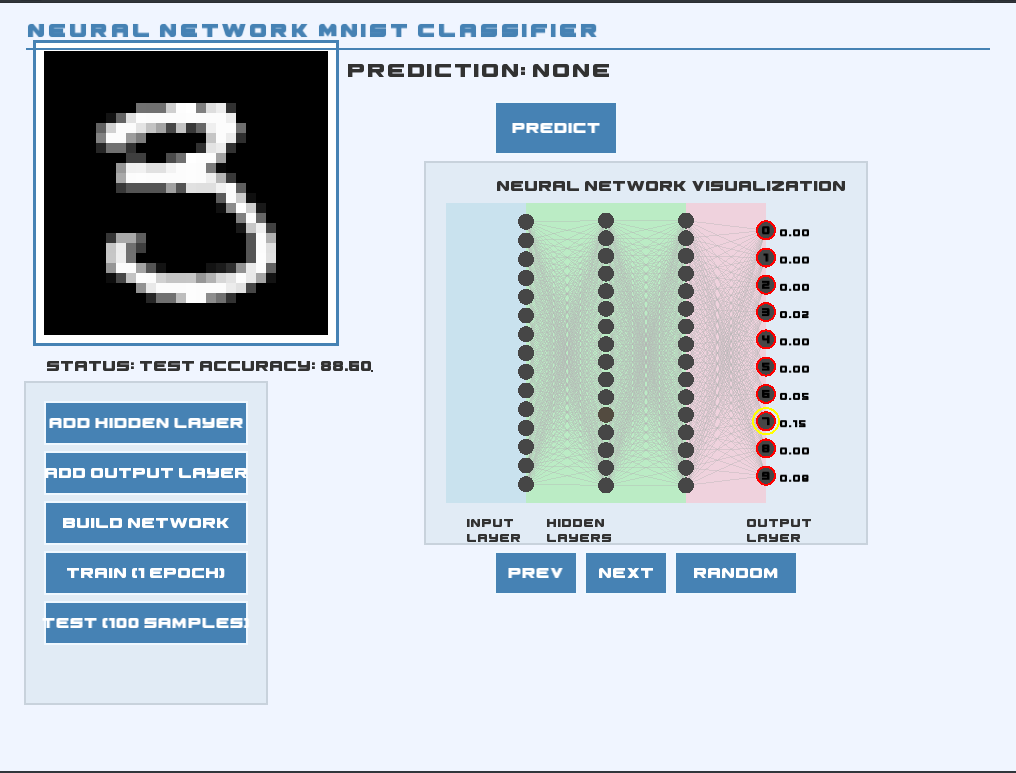
\includegraphics[width=0.8\textwidth]{test.png}
    \caption{Neural Network MNIST Classifier interface showing prediction and network visualization}
    \label{fig:test_interface}
\end{figure}

The implemented neural network classifier effectively demonstrates both the theoretical concepts of neural networks and the practical application of object-oriented programming principles. As shown in Figure \ref{fig:test_interface}, the user interface provides an intuitive way to interact with the neural network, visualize its structure, and observe predictions on MNIST digits. The test accuracy of 89.20\% indicates that the implementation achieves reasonable performance even with a relatively simple architecture.

\begin{lstlisting}[language=bash, caption=Shortened console output showing network structure and training progress]
$ ./NeuralNetworkMNIST
Network created
Loaded 100 images from data/mnist_data_test.csv
MNIST data loaded successfully

Calculating neuron positions for 4 layers
Neuron positions calculated. Layers: 4
  Layer 0: 15 neurons
  Layer 1: 16 neurons
  Layer 2: 16 neurons
  Layer 3: 10 neurons
Network visualization updated with 4 layers
Network structure finalized

Training on 2000 samples for 1 epochs...
Epoch 1/1, Loss: 2.28986
// ... training progress ...
Epoch 1/1, Loss: 0.429007
// ... further training ...
Epoch 1/1, Loss: 0.191356
// ... final training iterations ...
Epoch 1/1, Loss: 0.0441592
Training completed successfully

Test Accuracy: 89%, Loss: 0.552413
Test completed with accuracy: 89.00%
\end{lstlisting}

As shown in the console output above, the network was trained over multiple epochs with the loss steadily decreasing from 2.29 to 0.04, indicating successful learning. The final test accuracy of 89\% demonstrates the effectiveness of the implementation.

While the current implementation successfully meets the project objectives, there remain numerous opportunities for enhancement. The modular design allows for relatively straightforward integration of additional features such as convolutional layers, more sophisticated optimization techniques, enhanced visualization capabilities, and support for other datasets.\newline

In conclusion, this project demonstrates that principled object-oriented design is not just an academic exercise but a practical approach to managing complexity in real-world applications. By applying OOP concepts systematically, we have created a neural network implementation that is not only functional but also maintainable, extensible, and educational. The combination of a robust mathematical foundation with clean software design makes this project a valuable demonstration of how computer science theory and practice can effectively complement each other.

\subsection{Possible Enhancements}

Several potential enhancements could further improve the project:


\begin{itemize}
    \item Add support for saving and loading trained networks
    \item GPU acceleration for matrix operations can be used. 
    \item Implement visualizations of training progress (loss/accuracy graphs)
    \item Create a more detailed view of weight distributions
    \item Add more customization options for network architecture
\end{itemize}


\end{document} 